\chapter{模板(Stenciling)}
\begin{flushleft}
模板缓冲区是一个屏幕外缓冲区,我们可以使用它来实现一些特殊效果。 模板缓冲区具有与后缓冲区和深度缓冲区相同的分辨率,使得模板缓冲区中的第$i$个像素对应于后缓冲区和深度缓冲区中的第$i$个像素。 回想一下4.1.5,当指定模板缓冲区时,它会附加到深度缓冲区。 顾名思义,模板缓冲区用作模板,允许我们阻止某些像素片段渲染到后台缓冲区。\\

例如,在实现镜像时,我们需要在镜子的平面上反射一个物体; 但是,我们只想将反射绘制到镜子中。 我们可以使用模板缓冲区来阻止反射的渲染,除非它被绘制到镜像中(见图\ref{fig:11-1})。
\end{flushleft}

\begin{figure}[h]
    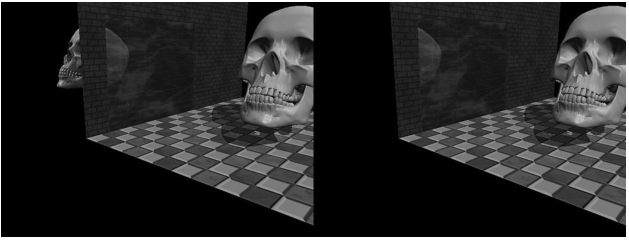
\includegraphics[width=\textwidth]{11-1}
    \centering
    \caption{(左)反射的头骨在镜子中正确显示。 墙体砖没有显示反射,因为它未能在该区域进行深度测试。 然而,在墙后面看,我们能够看到反射,从而打破了幻像(反射应该只通过镜子出现)。 (右)通过使用模板缓冲区,我们可以阻止反射的头骨被渲染,除非它被绘制在镜子中。}
    \label{fig:11-1}
\end{figure}

\begin{flushleft}
通过填写 D3D12\_DEPTH\_STENCIL\_DESC 实例并将其分配给管道状态对象(PSO)的 D3D12\_GRAPHICS\_PIPELINE\_STATE\_DESC::DepthStencilState 字段来配置模板缓冲区(以及深度缓冲区)状态。 通过研究现有的示例应用程序,学习有效地使用模板缓冲区。 一旦您了解了模板缓冲区的一些应用程序,您就可以更好地了解它如何用于您自己的特定需求。
{\large Objectives:}
\begin{itemize}
    \item 1.通过填写管道状态对象中的 D3D12\_DEPTH\_STENCIL\_DESC 字段来了解如何控制深度和模板缓冲区状态。
    \item 2.了解如何通过使用模板缓冲区来实现镜像,以防止反射被绘制到非镜像表面。
    \item 3.能够识别双重混合并理解模板缓冲区是如何防止它的。
    \item 4.解释深度复杂性,描述两种可以测量场景的深度复杂度的方式。
\end{itemize}
\end{flushleft}

%-------- 11.1 --------
\section{深度/模板格式和清除(Depth/Stencil Formats and Clearing)}
\begin{flushleft}
回忆深度/模板缓冲区是一种纹理,必须使用某些数据格式创建。用于深度/模板缓冲的格式如下:\\
\end{flushleft}

\begin{itemize}
  \item 1.DXGI\_FORMAT\_D32\_FLOAT\_S8X24\_UINT: 指定一个32位浮点型深度缓冲区,保留8位(无符号整数)用于映射到$[0,255]$范围的模板缓冲区,剩余24位不用于填充。
  \item 2.DXGI\_FORMAT\_D24\_UNORM\_S8\_UINT: 指定映射到$[0,1]$范围的无符号24位深度缓冲区,其中8位(无符号整数)保留给映射到$[0,255]$范围的模板缓冲区。
\end{itemize}

\begin{flushleft}
在我们的D3DApp框架中,当创建深度缓冲区时,指定:\\
\end{flushleft}

\begin{lstlisting}
DXGI_FORMAT mDepthStencilFormat = DXGI_FORMAT_D24_UNORM_S8_UINT;
depthStencilDesc.Format = mDepthStencilFormat;
\end{lstlisting}

\begin{flushleft}
此外,模板缓冲区应在每帧开始时重置为某个值。这是通过以下方法完成的(它也清除了深度缓冲区):\\
\end{flushleft}

\begin{lstlisting}
void ID3D12GraphicsCommandList::ClearDepthStencilView(
    D3D12_CPU_DESCRIPTOR_HANDLE DepthStencilView,
    D3D12_CLEAR_FLAGS ClearFlags,
    FLOAT Depth,
    UINT8 Stencil,
    UINT NumRects,
    const D3D12_RECT *pRects);
\end{lstlisting}

\begin{flushleft}
1.DepthStencilView: 我们想要清除深度/模板缓冲区视图的描述符。\\

2.ClearFlags: 指定 D3D12\_CLEAR\_FLAG\_DEPTH 仅清除深度缓冲区; 指定 D3D12\_CLEAR\_FLAG\_STENCIL 仅清除模板缓冲区; 指定 D3D12\_CLEAR\_FLAG\_DEPTH | D3D12\_CLEAR\_FLAG\_STENCIL 清除两者。\\

3.Depth: float-value 用于设置深度缓冲区中的每个像素; 它必须是浮点数$x$,$0\leq x\leq 1$。\\

4.Stencil: 用于设置模板缓冲区的每个像素的整数值; 它必须是整数$n$,$0\leq n\leq 255$。\\

5.NumRects: pRects指向的数组中的矩形数。\\

6.pRects: D3D12\_RECT 数组,用于标记深度/模板缓冲区上的矩形区域以进行清除; 指定 nullptr 以清除整个深度/模板缓冲区。\\
~\\
我们已经在演示的每个帧中调用了这个方法。:\\
mCommandList->ClearDepthStencilView(
    DepthStencilView(),
    D3D12_CLEAR_FLAG_DEPTH | D3D12_CLEAR_FLAG_STENCIL,
    1.0f, 0, 0, nullptr);
\end{flushleft}

%-------- 11.2 --------
\section{模板测试(The Stencil Test)}
\begin{flushleft}
如前所述,我们可以使用模板缓冲区来阻止渲染到后缓冲区的某些区域。 阻止特定像素被写入由模板测试决定,模板测试由以下内容给出:\\
\end{flushleft}

\begin{lstlisting}
if( StencilRef 
    & StencilReadMask Value 
    & StencilReadMask )
    accept pixel
else
    reject pixel
\end{lstlisting}

\begin{flushleft}
当像素被光栅化时(即,在输出合并阶段期间)执行模板测试,假设启用了模板,并采用两个操作数:\\

1.左侧(left-hand-side LHS)操作数,通过将应用程序定义的模板参考值(StencilRef)与应用程序定义的屏蔽值(StencilReadMask)进行AND运算确定。\\

2.右侧(right-hand-side RHS)操作数,通过对已经在模板缓冲区中的特定像素测试值(Value)与应用程序定义的屏蔽值(StencilReadMask)进行AND运算来确定。\\
~\\
请注意,LHS和RHS的StencilReadMask是相同的。 然后,模板测试将LHS与RHS进行比较,指定应用程序选择的比较函数,该函数返回true或false值。 如果测试结果为true,我们将像素写入后缓冲区(假设深度测试也通过)。 如果测试结果为false,那么我们阻止将像素写入后缓冲区。 当然,如果由于模板测试失败而导致像素被拒绝,则也不会将其写入深度缓冲区。\\

$\unlhd$操作符含义由下面枚举类定义:\\
\end{flushleft}

\begin{lstlisting}
typedef enum D3D12_COMPARISON_FUNC
{
    D3D12_COMPARISON_NEVER = 1,
    D3D12_COMPARISON_LESS = 2,
    D3D12_COMPARISON_EQUAL = 3,
    D3D12_COMPARISON_LESS_EQUAL = 4,
    D3D12_COMPARISON_GREATER = 5,
    D3D12_COMPARISON_NOT_EQUAL = 6,
    D3D12_COMPARISON_GREATER_EQUAL = 7,
    D3D12_COMPARISON_ALWAYS = 8,
} D3D12_COMPARISON_FUNC;
\end{lstlisting}
\begin{itemize}
  \item 1.D3D12\_COMPARISON\_NEVER:函数总是返回 false。
  \item 2.D3D12\_COMPARISON\_LESS:替换$\unlhd$为 $<$符号。
  \item 3.D3D12\_COMPARISON\_EQUAL:替换$\unlhd$为 $==$符号。
  \item 4.D3D12\_COMPARISON\_LESS\_EQUAL:替换$\unlhd$为 $\leq$符号。
  \item 5.D3D12\_COMPARISON\_GREATER:替换$\unlhd$为 $>$符号。
  \item 6.D3D12\_COMPARISON\_NOT\_EQUAL:替换$\unlhd$为 $!=$符号。
  \item 7.D3D12\_COMPARISON\_GREATER\_EQUAL:替换$\unlhd$为 $\geq$符号。
  \item 8.D3D12\_COMPARISON\_ALWAYS:函数总是返回 true。
\end{itemize}

%-------- 11.3 --------
\section{描述深度/模板状态(Describing The Depth/Stencil State)}
\begin{flushleft}
深度/模板状态由 D3D12\_DEPTH\_STENCIL\_DESC 实例填充定义:\\ 
\end{flushleft}

\begin{lstlisting}
typedef struct D3D12_DEPTH_STENCIL_DESC {
    BOOL DepthEnable; // Default True
    // Default: D3D11_DEPTH_WRITE_MASK_ALL
     D3D12_DEPTH_WRITE_MASK DepthWriteMask;
    // Default: D3D11_COMPARISON_LESS
    D3D12_COMPARISON_FUNC DepthFunc;
    BOOL StencilEnable; // Default: False
    UINT8 StencilReadMask; // Default: 0xff
    UINT8 StencilWriteMask; // Default: 0xff
    D3D12_DEPTH_STENCILOP_DESC FrontFace;
    D3D12_DEPTH_STENCILOP_DESC BackFace;
} D3D12_DEPTH_STENCIL_DESC;
\end{lstlisting}

%-------- 11.3.1 --------
\subsection{深度设置(Depth Settings)}
\begin{flushleft}
1.DepthEnable: 指定true以启用深度缓冲; 指定false以禁用它。 禁用深度测试时,绘制顺序很重要,即使它位于遮挡对象后面,也会绘制像素片段(回顾4.1.5)。 如果禁用深度缓冲,则无论DepthWriteMask设置如何,深度缓冲区中的元素也不会更新。\\

2.DepthWriteMask: 这可以是 D3D12\_DEPTH\_WRITE\_MASK\_ZERO 或 D3D12\_DEPTH\_WRITE\_MASK\_ALL,但不能同时使用两者。假设 DepthEnable 设置为 true,D3D12\_DEPTH\_WRITE\_MASK\_ZERO禁用对深度缓冲区的写入,但仍会进行深度测试。D3D12\_DEPTH\_WRITE\_MASK\_ALL允许写入深度缓冲区; 如果深度和模板测试都通过,将写入新的深度。 控制深度读取和写入的能力对于实现某些特殊效果是必要的。\\

3.DepthFunc: 指定 D3D12\_COMPARISON\_FUNC 枚举类型的成员之一以定义深度测试比较功能。 通常这总是 D3D12\_COMPARISON\_LESS,以便执行通常的深度测试,如4.1.5中所述。 也就是说,如果像素片段的深度值小于写入后缓冲器的前一像素的深度,则接受该像素片段。 但正如您所看到的,Direct3D允许您在必要时自定义深度测试。\\
\end{flushleft}

%-------- 11.3.2 --------
\subsection{模板设置(Stencil Settings)}
\begin{flushleft}
1.
\end{flushleft}



